\documentclass[a4paper,10pt,twoside]{article}

%===========PACOTES
\usepackage[body={165mm,235mm}]{geometry}
%\usepackage[portuguese]{babel}
\usepackage{a1}
\usepackage[english]{babel}
\usepackage[latin1]{inputenc} %permite o uso de acentos
%\usepackage[dvips]{color}
\usepackage{amsfonts,amssymb}
%\usepackage{epsfig}
\usepackage{amsmath}
\usepackage{graphicx}	

% makeidx
\usepackage{makeidx}
% make index
\makeindex
%\usepackage[pdftex]{graphicx}


\def\mapright#1#2#3{\smash{\mathop{\hbox to
#3{\rightarrowfill}}\limits^{#1}_{#2}}}

\def\mapleft#1#2#3{\smash{\mathop{\hbox to
#3{\leftarrowfill}}\limits^{#1}_{#2}}}

\def\mapright#1#2{\smash{\mathop{\hbox to 0.90cm{\rightarrowfill}}\limits^{#1}_{#2}}}
\def\mapleft#1#2{\smash{\mathop{\hbox to 0.90cm{\leftarrowfill}}\limits^{#1}_{#2}}}

\def\mapleftright#1#2{\smash{\mathop{\hbox to 0.80cm{\leftarrowfill \rightarrowfill}}\limits^{#1}_{#2}}}
\def\ext{\times \! \vrule depth0pt height5pt width0.35pt}

\def\H{\mathcal H}
\def\D{\mathcal D}
\def\B{\mathcal B}
\def\C{\mathbb C}
\def\R{\mathbb R}
\def\S{\mathbb S}
\def\U{\mathcal U}
\def\Z{\mathbb Z}

\title{All the shapes of spaces: a census of 9-small 3-manifolds
\footnote{2010 Mathematics Subject Classification: 
57M25 and 57Q15 (primary), 57M27 and 57M15 (secondary)}} 
\author{S�stenes L. Lins and Lauro D. Lins}

\date{\today}


\begin{document}


\maketitle
\begin{abstract}


In this work we present a complete (no misses, no duplicates) catalogue for closed, orientable and
prime 3-manifolds induced by plane graphs with a 
bipartition of its edge set (blinks) up to 9 edges. Blinks form a universal encoding for such manifolds. 
We hope that this census becomes as useful for the study of concrete examples of 3-manifolds
as the tables of knots are in the study of knots and links. Along the years we have made an issue
in our computational work that it must be reproducible and independently checked by other researchers. 
Our software is available,
but currently it lacks yet a good documentation and help is welcome to change this. An Wiki open source project
is starting.


\end{abstract}
\section{Introduction} 

John Hempel in his book {\em 3-Manifolds} \cite{hempel1976} said in opening Section 15 on Open Problems:\\
``The ultimate goal of the theory would be in providing solutions to:
 {\em The homeomorphism problem}: provide an {\em effective} procedure
 for determining whether two {\em given} 3-manifolds are homeomorphic, together with
 {\em The classification problem}: {\em effectively} generate a list containing
 exactly one 3-manifold from each homeomorphism class.'' We here provide a road for a 
 segmented answer for these questions. The closed oriented 3-manifolds are partitioned
 by the number of edges in a minimum encoding of them by a certain class of plane graphs, shortly
 to be defined. We use lexicography to define a representative unique plane graph for each 3-manifold
 of that type. We explicitly solve the segmented problem up to 9 edges, see Theorem \ref{theorem:census9}.

 This work is in the confluency of two deep research passions of the authors, apparently very far apart:
 The study of closed orientable 3-manifolds and the study of plane 
 graphs. By putting a bit of combinatorics
 on the graphs, namely, partitioning their edges into black and gray in an arbitrary way 
 we get an object named a {\em blink}.
 We make here explicitly that each class of homeomorphic closed oriented 3-manifolds is a subtle class
 of blinks where two membres of each class is linked by means of a small sets of local simple moves. 
 Thus, as simple as the blinks are, nevertheless they hold the mystery of 3-manifolds in their gist.
 
 
In references \cite{kauffman1994tlr}, \cite{lins2007blink} and \cite{lins1995gca}
we have defined and show how a {\em blink}, that is, a plane graph with
an arbitrary partition of its edges (here presented as colors black and gray) induces a well
defined closed oriented 3-manifold. Moreover each such a manifold is induced by a blink (in fact, by infinite blinks).
An {\em $n$-small} is a closed, orientable, and prime
3-manifold is a manifold induced by a blink with at most $n$ edges.
Relative to \cite{lins2007blink} the blinks of next theorem have receive two additions, the representative blinks
$U[1563]$ and $U[2165]$.
This is because the HGnQI-classes $9_{126}$ and $9_{199}$ of \cite{lins2007blink} split
into two topological classes. An objective of the present work is to prove that the splitings indeed take place.

We observe that the blinks are enlarged in the appendix, showing them together with the
corresponding blackboard framed links. The notation $n_i$ attached to each blink below,
is the name of its homeomorphism class, not merely its hgqi-class, as in \cite{lins2007blink}. 
\eject
\noindent
This paper concludes the proof of the following theorem: 
\begin{theorem}
Let $M^3$ be a closed, oriented and prime 3-manifold induced by a blink with at most 9 edges.
Then $M^3$ is homeomorphic to exactly one of the 
3-manifolds induced by the 489  blinks below. Morever all of these are pairwise non-homeomorphic.\\
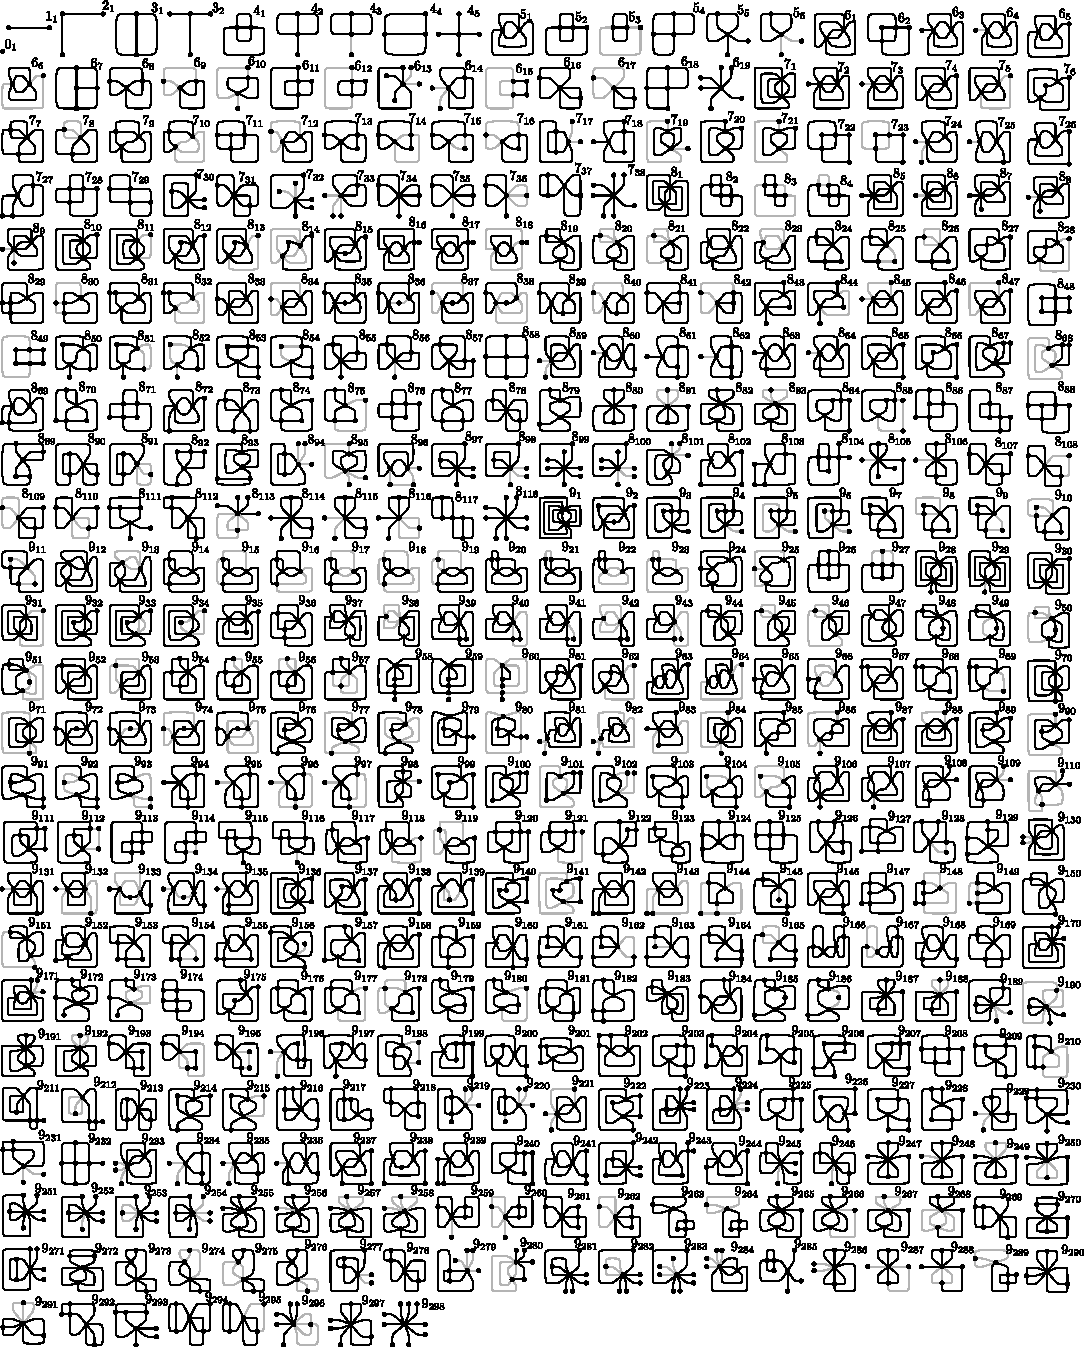
\includegraphics[width=16.8cm]{A.figs/primes489.pdf}
\label{theorem:census9}
\end{theorem}

\begin{proof}
 The proof follows from L.Lins' thesis and from the discussion about the lengths of the
 smallest geodesics of the classes $9_{126}$ and $9_{199}$
\end{proof}

\section{The resolution of the doubts left in L. Lins' thesis}
The topological classification of the 9-small spaces was nearly completed in 
\cite{lins2007blink}. This work develops a theory for generating a distinguished
set of blinks named $U_n$ and indexed lexicographically, $U_n[i]$ is the $i$-th such blink.
The relevance of $U_n$ is that it misses no closed, orientable, prime and irreducible
3-manifold which is induced by a blink with $n$-edges. 

The 3-manifolds of \cite{lins2007blink} are classified by homology and the quantum WRT$_r$-invariants
$r=3,\ldots,u$, up to $d$ decimal digits forming $hgqi_u^d$-classes. Our algorithm for computing the 
$WRT_r^d$-invariants are based on the theory developed in \cite{kauffman1994tlr}.

 
 \begin{figure}[!h]
\begin{center}
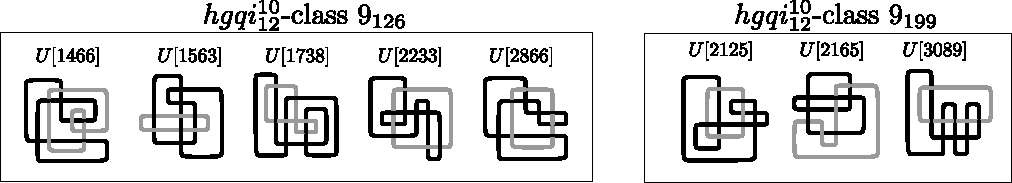
\includegraphics[width=16cm]{A.figs/nine126nine199.pdf}
\caption{\sf {\bf Note's final challenge:}  classify topologically $9_{126}$ and $9_{199}$. 
Here, to classify has the following strict meaning: for each pair}
\label{fig:nine126nine199}
\end{center}
\end{figure} 


After 6 years we have put our doubts as a Challenge to topologists and 
group algebraists, \cite{linslins2013A}.
\cite{weeks2001snappea}

 
 \begin{figure}
\begin{center}
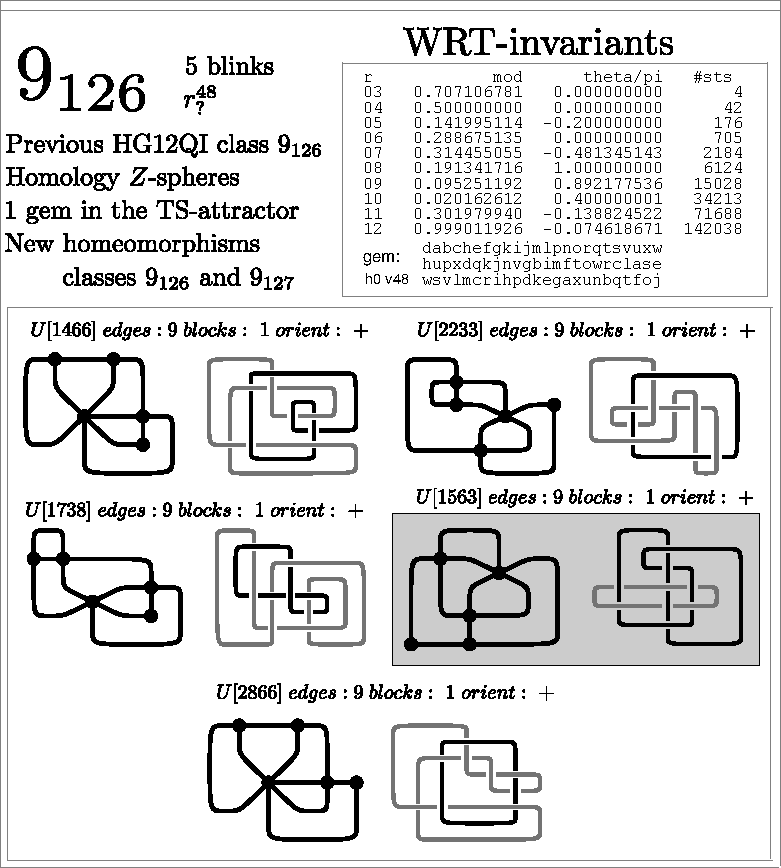
\includegraphics[width=8.0cm]{A.figs/nine126.pdf}
\caption{\sf {\bf Note's final challenge:}  classify topologically $9_{126}$ and $9_{199}$. 
Here, to classify has the following strict meaning: for each pair}
\label{fig:nine126}
\end{center}
\end{figure} 

 \begin{figure}
\begin{center}
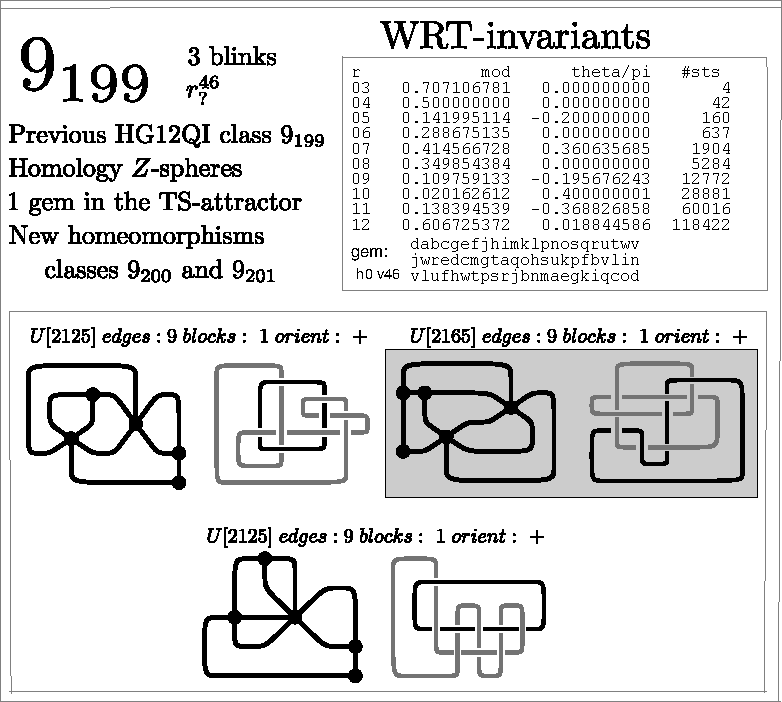
\includegraphics[width=8.0cm]{A.figs/nine199.pdf}
\caption{\sf {\bf Note's final challenge:}  classify topologically $9_{126}$ and $9_{199}$. 
Here, to classify has the following strict meaning: for each pair}
\label{fig:nine199}
\end{center}
\end{figure} 

\eject
\section{Appendix: census (no misses, no duplicates) of 9-small 3-manifolds}

\subsection*{Part 1/4 in terms of blinks:}
\center{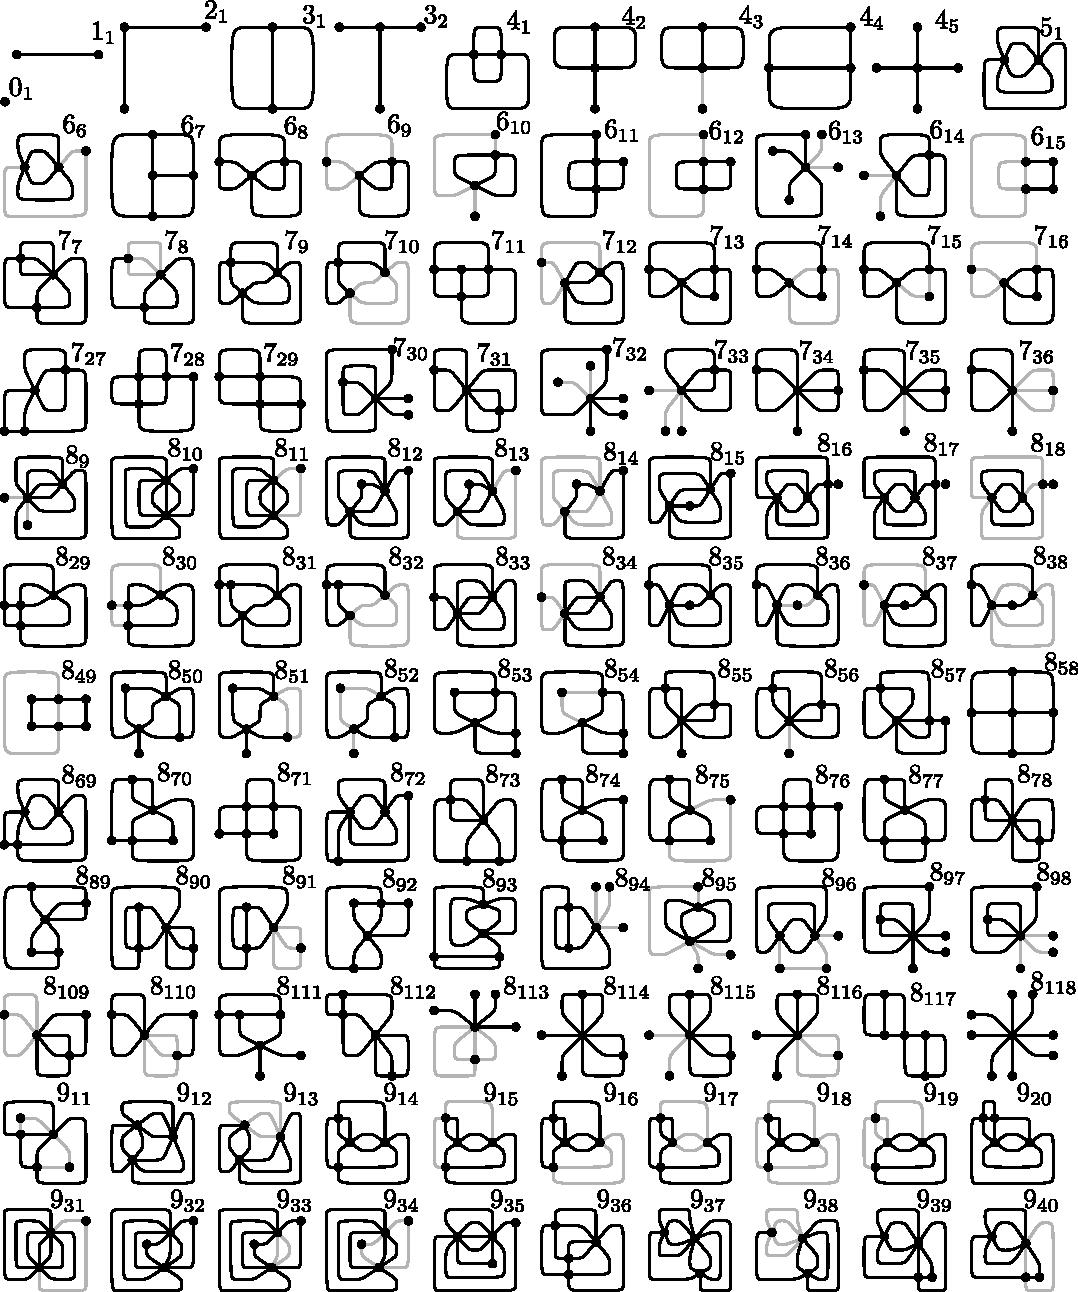
\includegraphics[width=16.5cm]{A.figs/primes489m11.pdf}} \eject \noindent
\subsection*{Part 1/4 in terms of blackboard framed links:}
\center{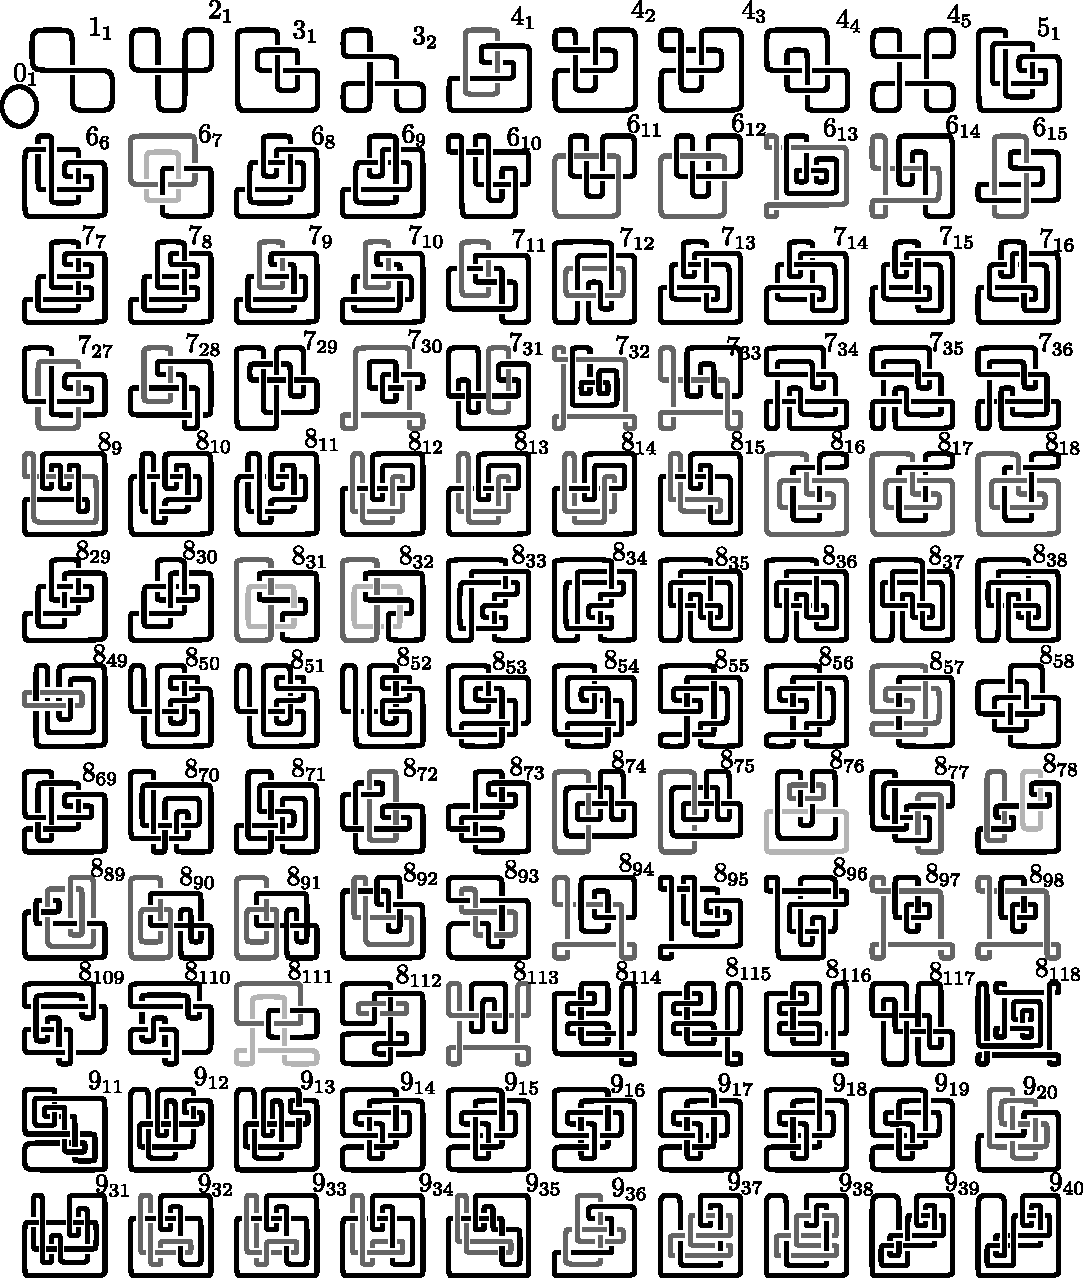
\includegraphics[width=16.5cm]{A.figs/primes489linksm11.pdf}} \eject
\subsection*{Part 2/4 in terms of blinks:}
\center{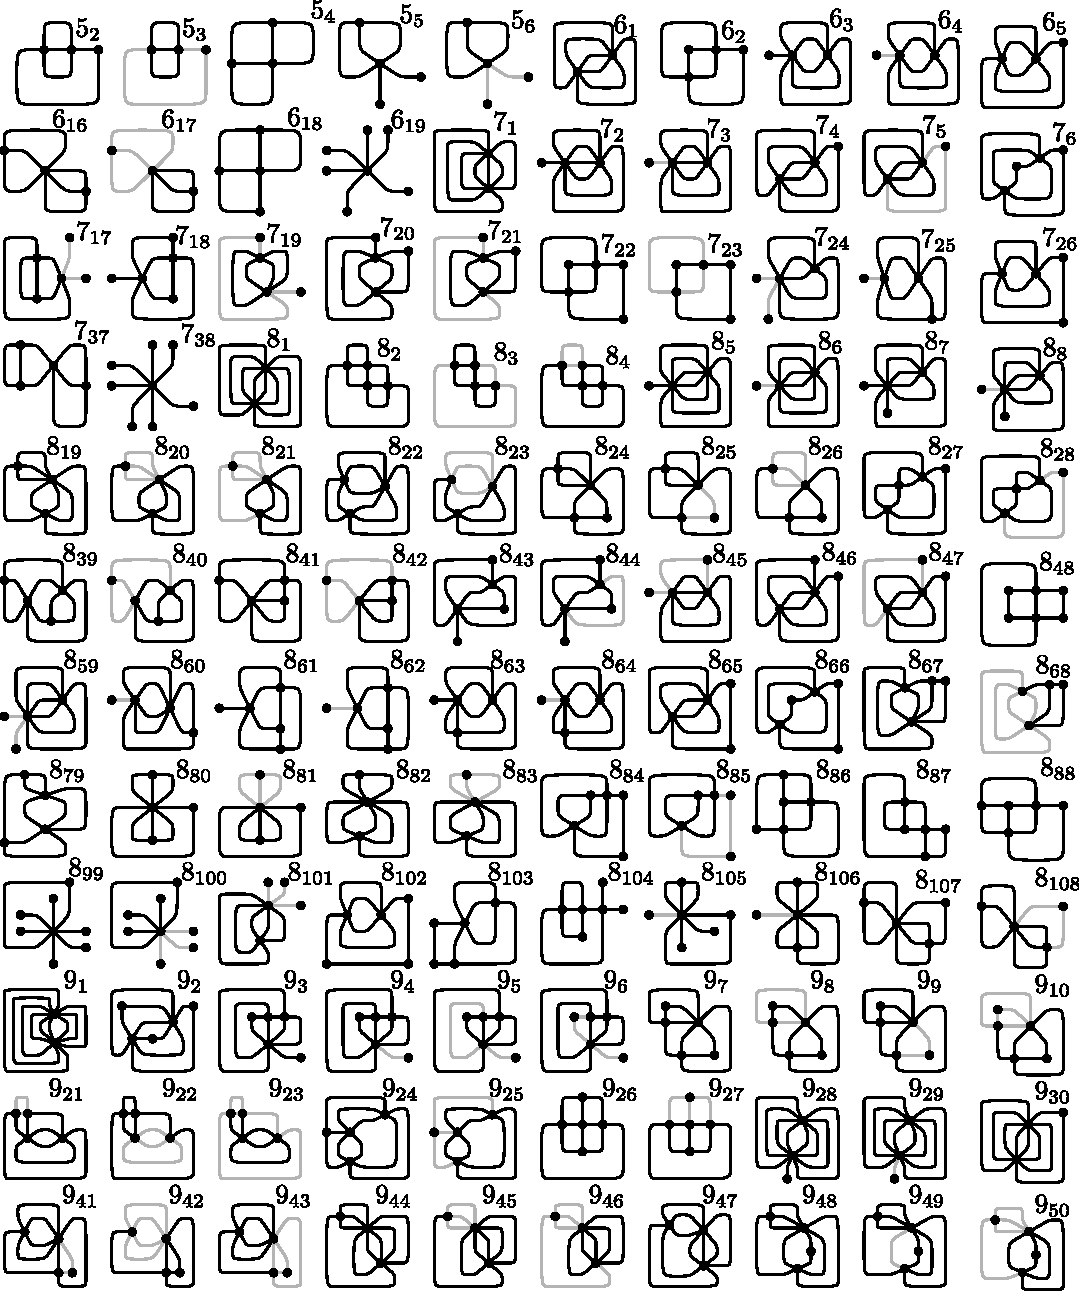
\includegraphics[width=16.5cm]{A.figs/primes489m12.pdf}} \eject
\subsection*{Part 2/4 in terms of blackboard framed links:}
\center{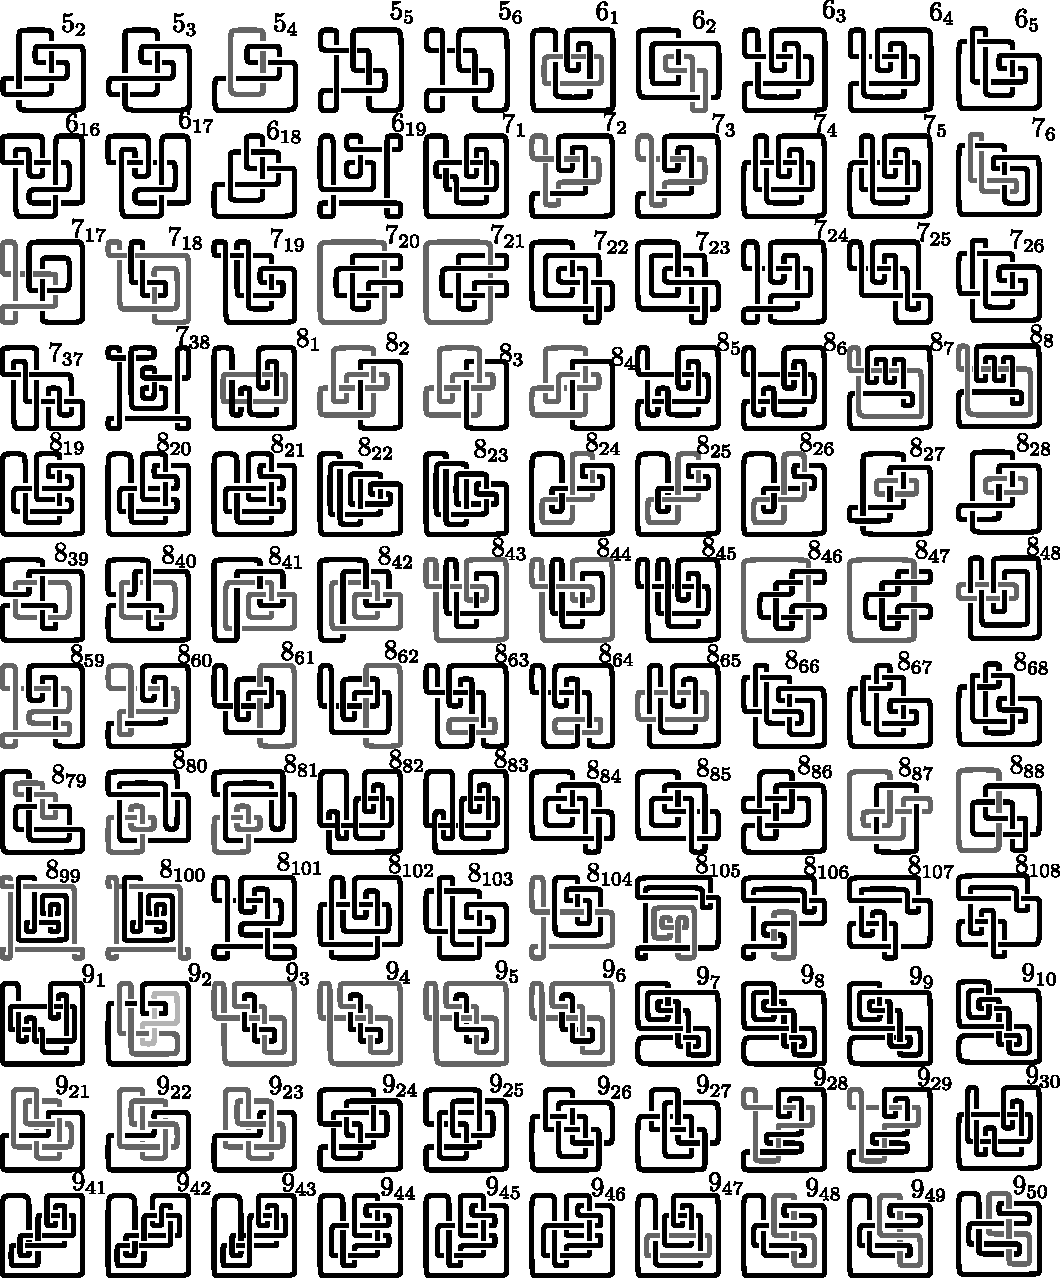
\includegraphics[width=16.5cm]{A.figs/primes489linksm12.pdf}} \eject
\subsection*{Part 3/4 in terms of blinks:}
\center{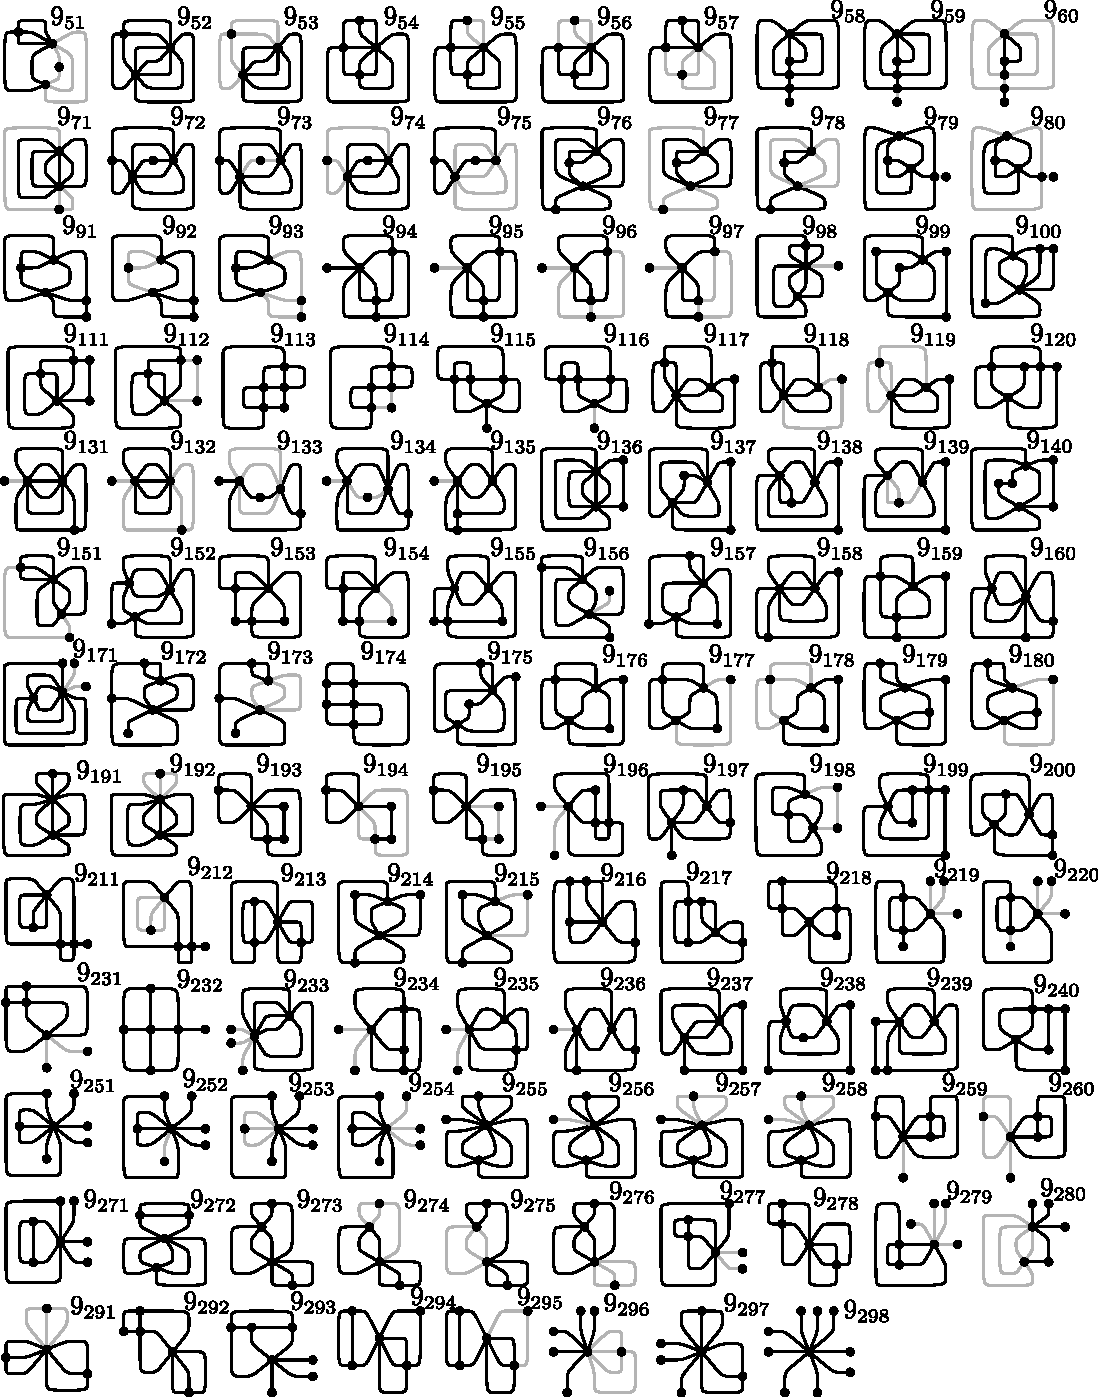
\includegraphics[width=16.5cm]{A.figs/primes489m21.pdf}} \eject
\subsection*{Part 3/4 in terms of blackboard framed links:}
\center{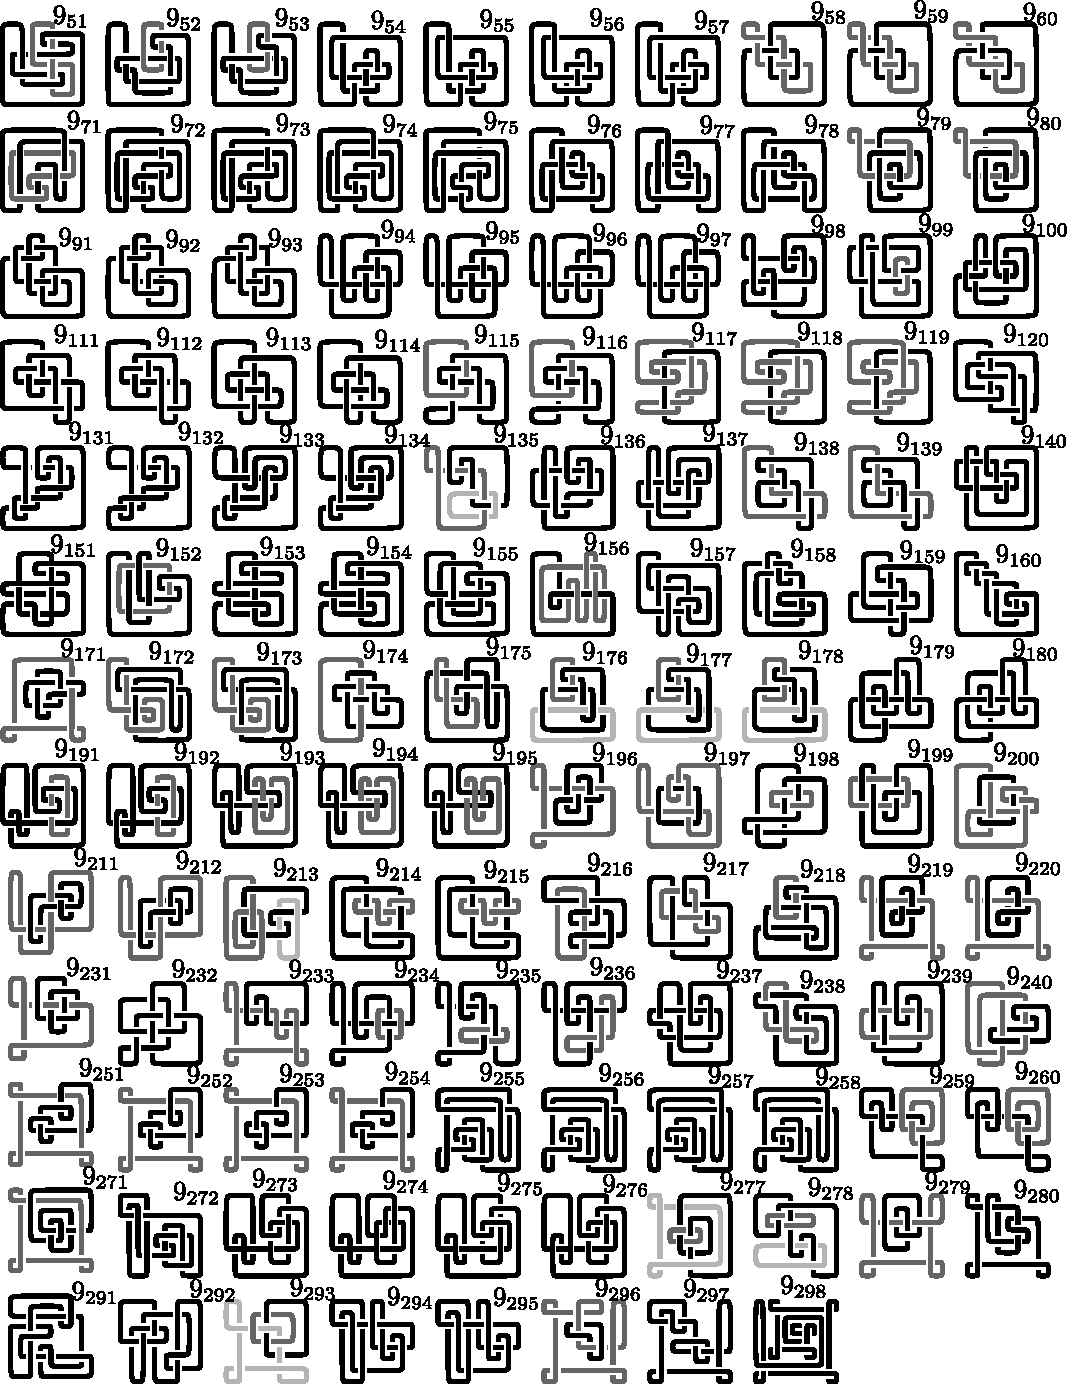
\includegraphics[width=16.5cm]{A.figs/primes489linksm21.pdf}} \eject
\subsection*{Part 4/4 in terms of blinks:}
\center{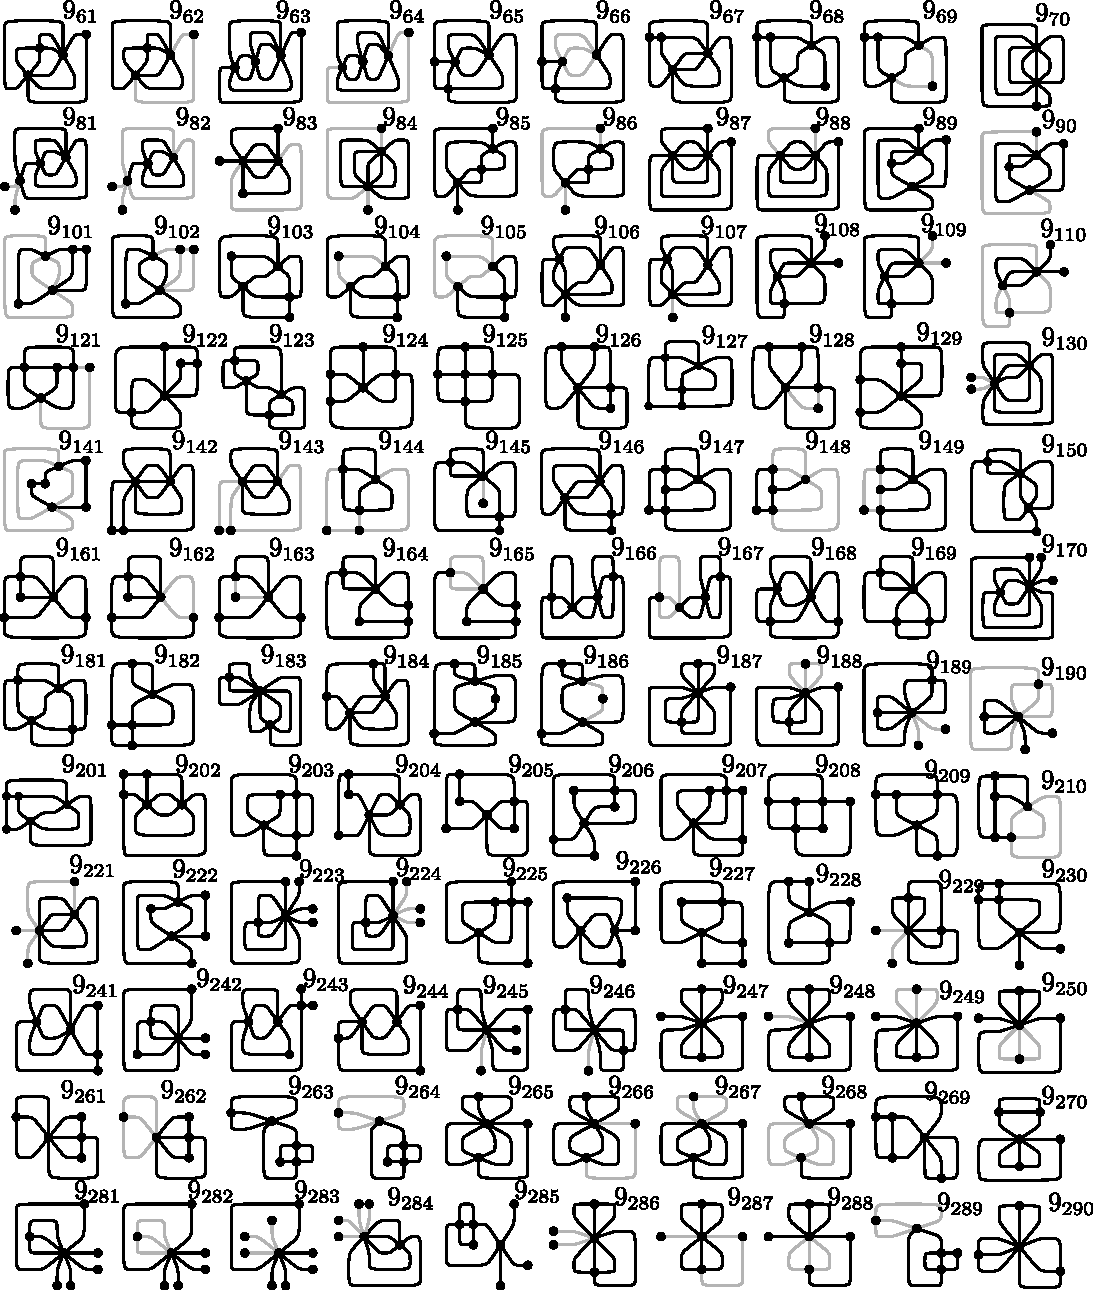
\includegraphics[width=16.5cm]{A.figs/primes489m22.pdf}} \eject
\subsection*{Part 4/4 in terms of blackboard framed links:}
\center{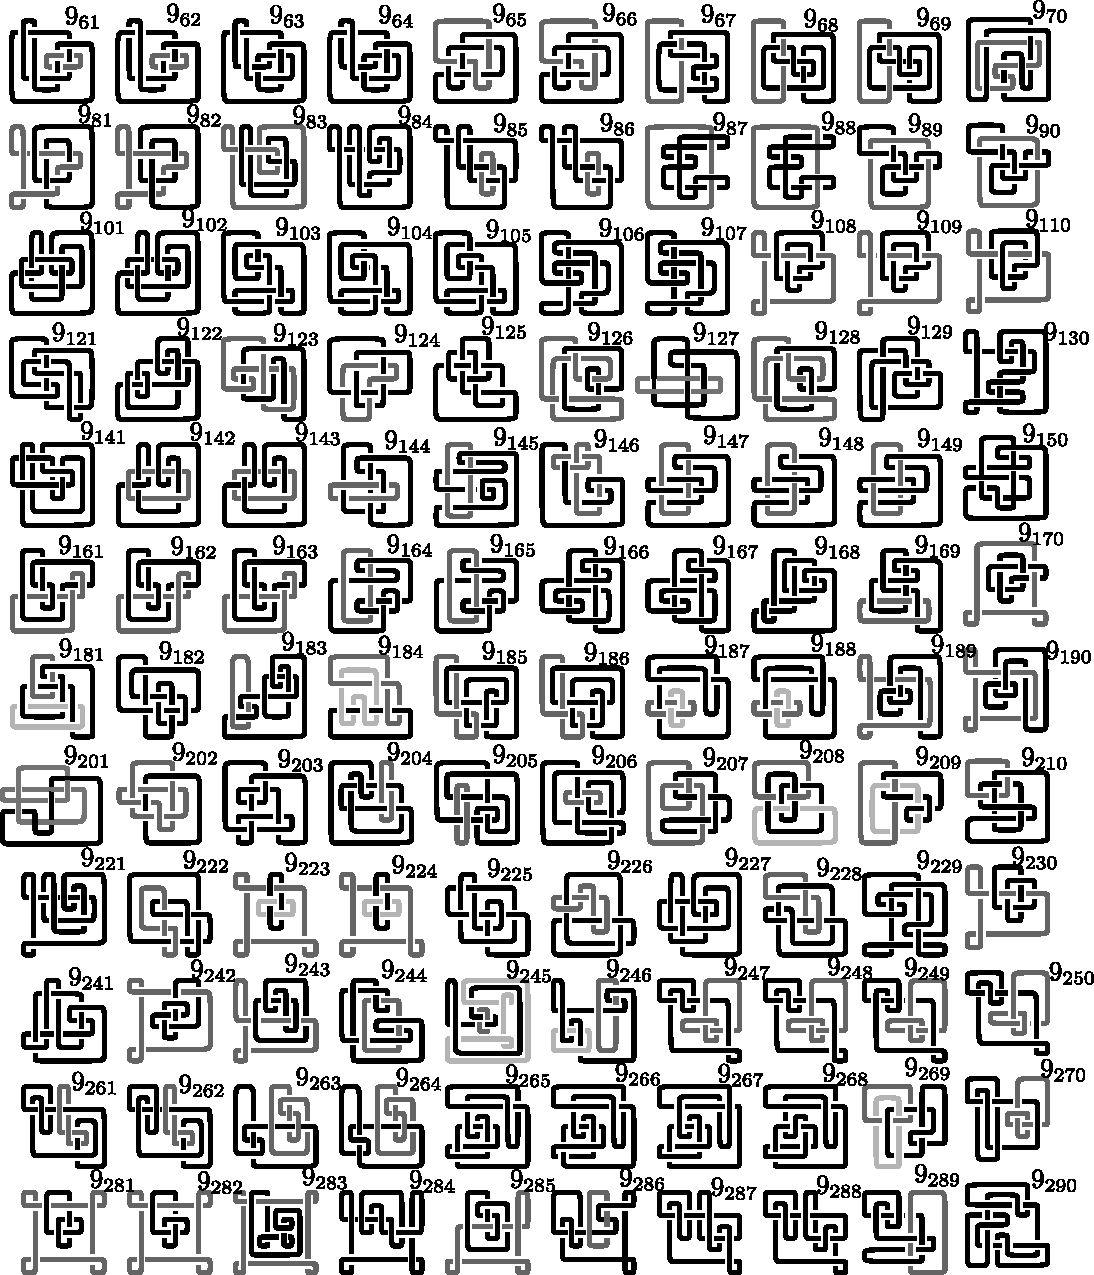
\includegraphics[width=16.5cm]{A.figs/primes489linksm22.pdf}} \eject


%-----------------------------------
%-----------------------------------

\section{Definition of Gem}
For completeness we briefly recall the basic definitions of gem theory, leading to its definition, \cite{lins1995gca}.
A {\em 4-graph} $G$ is a finite bipartite 4-regular graph whose edges are partitioned into 4 colors,
0,1,2, and 3, 
so that at each vertex there is an edge of each color, a proper edge-coloration, \cite{bondy1976gta}.
For each $i \in \{0,1,2,3\}$, let $E_i$ denote the set of $i$-colored edges of $G$.
A $\{j,k\}$-residue in a $4$-graph $G$ is a connected component of the subgraph induced by $E_j \cup E_k$.
A 2-residue is a $\{j,k\}$-residue, for some distinct colors $j$ and $k$.
A {\em gem} is a 4-graph $G$ such that for each color $i$, $G\backslash E_i$ can be embedded in the plane 
such that the boundary of each face is a 2-residue. From a gem there exists a straightforward
algorithm to obtain a closed orientable 3-manifold, in two different, dual ways. Every such a manifold is obtainable in this way.
An unecessary big gem is obtained from a triangulation $T$ for a manifold by taking the dual of the 
barycentric subdivision of $T$. Here the colors corresponds to the dimensions. Doing simplifications in the gem
completely destroys this correspondence.

\section{Conclusion}
A closed orientable 3-manifold is denoted {\em $n$-small} if it is induced by surgery on
a blackboard framed link with at most $n$ crossings.
Our bet is that both pairs of 3-manifolds in the 2 first sections of 
this short note are not homeomorphic. This would mean that the $9$-small manifolds are
completely classified and that
the combinatorial dynamics of Chapter 4 in \cite{lins1995gca} based 
on $TS$-moves which leads to a  (small, in the case of hyperbolic 3-manifolds)
number of minimal gems, named the {\em attractor of
the 3-manifold} is successful. This induces an efficient algorithm which 
is capable of classifying topologically all the 3-manifolds given as a blackboard framed link
with up to (so far) 9 crossings and maintains live the two Conjectures of page 15 of \cite{lins1995gca}:
the $TS$- and $u^n$-moves yield an efficient algorithm
to classify $n$-small 3-manifolds by explicitly displaying homeomorphisms, whenever they exist.


%-----------------------------------
\bibliographystyle{plain}
%\bibliographystyle{is-alpha}
%\addcontentsline{toc}{bibliografia}{\MakeTextUppercase{Refer�ncias Bibliogr�ficas}}
%\bibliography{d:/slsl\3.DadosSostenes.35.ArtigosLivros.bibtexGoogleScholar/bibtexIndex.bib} % bib file is slsl.bib
%\bibliography{~/home/ricardo/Dropbox/35.ArtigosLivros.bibtexGoogleScholar/bibtexIndex.bib}
\bibliography{bibtexIndex.bib}
%\bibliography{slsl}


\vspace{5mm}
\begin{center}
\hspace{7mm}
\begin{tabular}{l}
   S\'ostenes L. Lins\\
   Centro de Inform\'atica, UFPE \\
   Av. Jornalista Anibal Fernandes s/n\\
   Recife, PE 50740-560 \\
   Brazil\\
   sostenes@cin.ufpe.br
\end{tabular}
\hspace{20mm}
\hspace{7mm}
\begin{tabular}{l}
Lauro D. Lins\\
AT\&T Labs Research \\
180 Park Avenue \\
Florham Park, NJ 07932 \\
USA\\
llins@research.att.com
\end{tabular}
\hspace{20mm}

\end{center}


\end{document}

\begin{figure}[!htb]
\begin{center}
\includegraphics[scale=0.8]{A.figs/seconddoubt.pdf}
\caption{Are these 3-manifolds homeomorphic?}
\label{fig:seconddoubt}
\end{center}
\end{figure}

% \printindex
